\documentclass[convert={density=300,outext=.png}]{standalone}
\usepackage{tikz}

\begin{document}
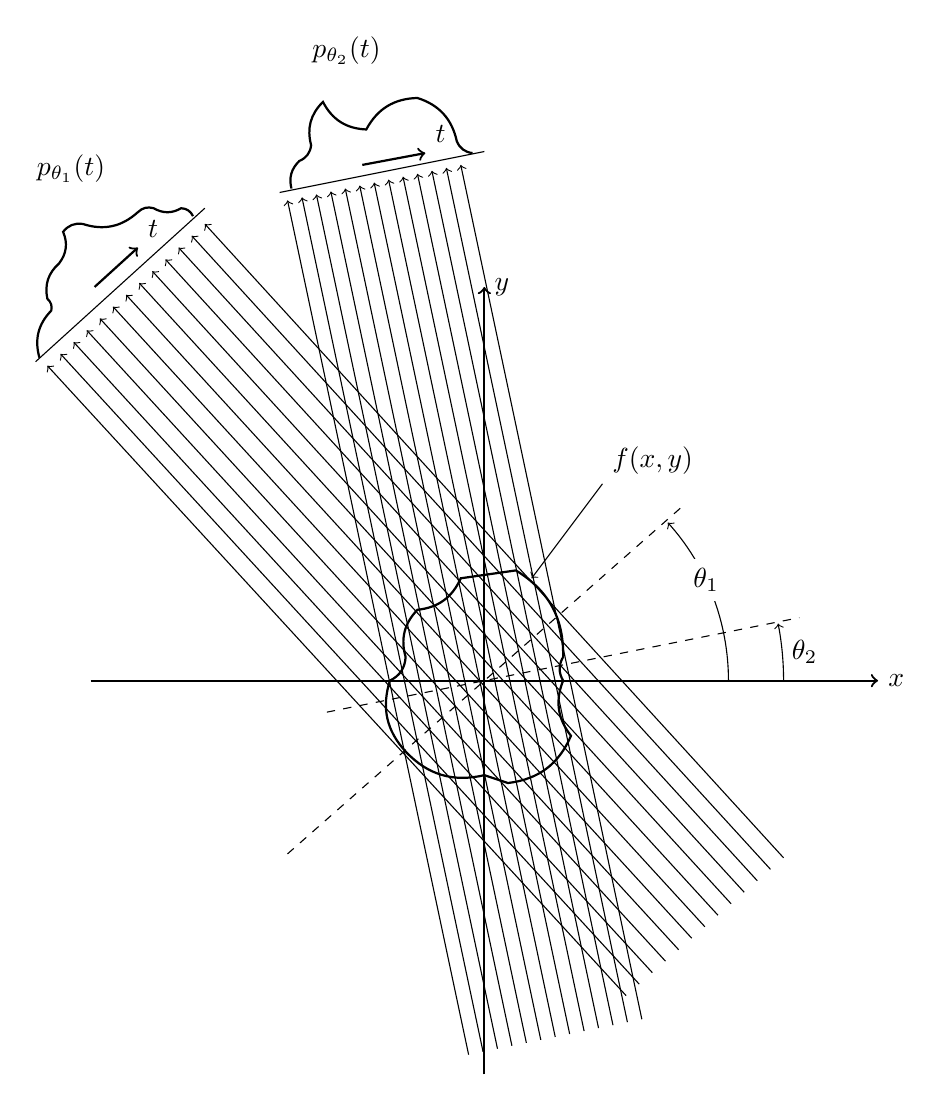
\begin{tikzpicture}[axis/.style={thick,->}]
    \draw[axis] (-5, 0) -- (5, 0) node [right] {$x$};
    \draw[axis] (0, -5) -- (0, 5) node [right] {$y$};

    % Objekt
    \draw[thick] (1, 0) to [bend left] (1, 0.3) to [bend right] (0.4, 1.4) to (-0.3, 1.3)
                 to [bend left] (-0.85, 0.9) to [bend right] (-1, 0.3) to [bend left] (-1.2, 0)
                 to [bend right] (-1, -0.9) to [bend right] (0, -1.2) to (0.3, -1.3) to [bend right] (1.1 ,-0.7)
                 to [bend left] (1, 0);
    \draw[->] (1.5, 2.5) -- (0.6, 1.3) node [pos=0, above right] {$f(x, y)$};

    % Detektorebenen
    \draw[dashed] (-2.5, -2.2) -- (2.5, 2.2);
    \draw[dashed] (-2, -0.4) -- (4, 0.8);

    % Detektor 1
    \draw (-5.7, 4.05) -- (-3.55, 6);
    \draw[axis] (-4.95, 5) -- (-4.4, 5.5) node [sloped, above right] {$t$};
    \draw[thick] (-5.65, 4.1) to [bend left] (-5.5, 4.7) to [bend right] (-5.55, 4.85)
                              to [bend left] (-5.4, 5.3) to [bend right] (-5.35, 5.7)
                              to [bend left] (-5.1, 5.8) to [bend right] (-4.4, 5.95)
                              to [bend left] (-4.2, 6) to [bend right] (-3.85, 6)
                              to [bend left] (-3.7, 5.9);
    \node at (-5.25, 6.5) {$p_{\theta_1}(t)$};

    % Strahlen zu Detektor 1
    \foreach \w in {0,...,12}
        \draw [->] (1.8 + \w * 0.16666666666667, -4 + \w * 0.14583333333333)
                    -- (-5.55 + \w * 0.16666666666667, 4 + \w * 0.15);

    % Detektor 2
    \draw (-2.6, 6.2) -- (0, 6.72);
    \draw[axis] (-1.55, 6.55) -- (-0.75, 6.7) node [above right] {$t$};
    \draw[thick] (-2.45, 6.25) to [bend left] (-2.35, 6.6) to [bend right] (-2.2, 6.8)
                               to [bend left] (-2.05, 7.35) to [bend right] (-1.5, 7)
                               to [bend left] (-0.85, 7.4) to [bend left] (-0.35, 6.85)
                               to [bend right] (-0.15, 6.7);
    \node at (-1.75, 8) {$p_{\theta_2}(t)$};

    % Strahlen zu Detektor 2
    \foreach \w in {0,...,12}
        \draw [->] (-0.2 + \w * 0.1833333333333, -4.75 + \w * 0.0375)
                    -- (-2.5 + \w * 0.1833333333333, 6.1 + \w * 0.0375);

    % Winkel
    \draw [->] (3.1, 0) arc (0:42:30mm) node [pos=0.6, fill=white] {$\theta_1$};
    \draw [->] (3.8, 0) arc (0:11:38mm) node [pos=0.5, right] {$\theta_2$};
\end{tikzpicture}
\end{document}
